
\goodbreak
\newpage
\clearpage
\section{MÉTODOS ÁGEIS}
A muito tempo vários métodos para desenvolvimento de software são propostos. 
Em 2001, um grupo de pessoas muito experientes em desenvolvimento de software, juntaram-se em Salt Lake City, Utah, para resolverem problemas de desenvolvimento de software \cite{Greene2014}.
Como resultado deste encontro, foi criado o manifesto ágil, que é reproduzido a seguir \cite{Beck2001}:

\begin{citacao}

Estamos descobrindo maneiras melhores de desenvolver software, fazendo-o nós mesmos e ajudando outros a fazerem o mesmo. 
Através deste trabalho, passamos a valorizar:

Indivíduos e interações mais que processos e ferramentas;

Software em funcionamento mais que documentação abrangente;

Colaboração com o cliente mais que negociação de contratos;

Responder a mudanças mais que seguir um plano.

Ou seja, mesmo havendo valor nos itens à direita, valorizamos mais os itens à esquerda.
\end{citacao}

Meses após a criação do manifesto, estas pessoas também criaram os princípios ágeis e a Aliança Ágil \cite{Layton2012}.

Os princípios ágeis são um conjunto de 12 itens com o objetivo de auxiliar na implantação de metodologias ágeis. Eles são reproduzidos a seguir a título de ilustração \cite{Beck2001}:

\begin{citacao}
		1. Nossa maior prioridade é satisfazer o cliente
		através da entrega contínua e adiantada
		de software com valor agregado.

		2. Mudanças nos requisitos são bem-vindas,
		mesmo tardiamente no desenvolvimento.
		Processos ágeis tiram vantagem das
		mudanças visando vantagem competitiva para o cliente.

		3. Entregar frequentemente software funcionando,
		de poucas semanas a poucos meses,
		com preferência à menor escala de tempo.

		4. Pessoas de negócio e desenvolvedores devem trabalhar
		diariamente em conjunto por todo o projeto.

		5. Construa projetos em torno de indivíduos motivados.
		Dê a eles o ambiente e o suporte necessário
		e confie neles para fazer o trabalho.

		6. O método mais eficiente e eficaz de transmitir
		informações para e entre uma equipe de desenvolvimento
		é através de conversa face a face.

		7. Software funcionando é a medida primária de progresso.

		8. Os processos ágeis promovem desenvolvimento
		sustentável. Os patrocinadores, desenvolvedores e
		usuários devem ser capazes de manter um ritmo
		constante indefinidamente.

		9. Contínua atenção à excelência técnica e bom design
		aumenta a agilidade.

		10. Simplicidade--a arte de maximizar a quantidade de
		trabalho não realizado--é essencial.

		11. As melhores arquiteturas, requisitos e designs
		emergem de equipes auto-organizáveis.

		12. Em intervalos regulares, a equipe reflete sobre como
		se tornar mais eficaz e então refina e ajusta seu
		comportamento de acordo. 
\end{citacao}

Este manifesto serviu de marco agregador de métodos e técnicas, que já existiam a época, mas não eram amplamente difundidas como \emph{Scrum}, \emph{Extreme Programming}, \emph{kanban}, \emph{lean}, entre outros. 
Estas técnicas, apesar de anteriores ao manifesto, possuem em seus cernes, muito em comum com os valores ágeis.
A Figura \ref{cap2_valores} tenta ilustrar esta ideia.
\begin{figure}[ht]
	\centering
	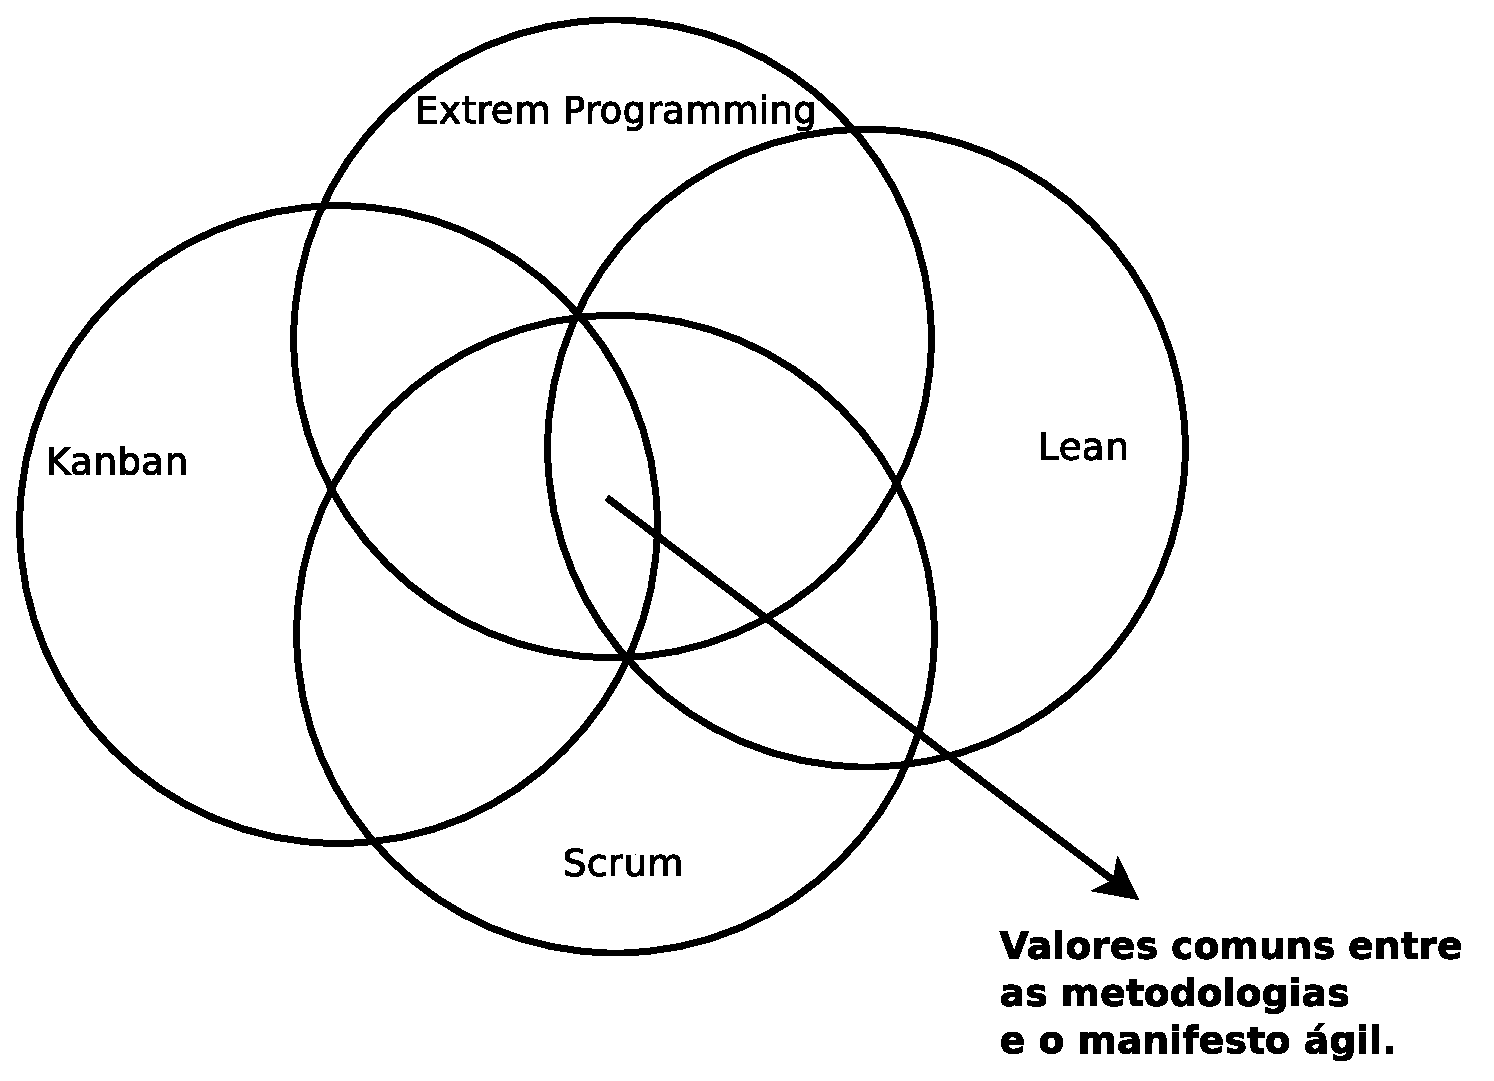
\includegraphics[width=7cm]{figuras/cap2_valores.eps}
	\caption{Valores em comum. Adaptado de \cite{Greene2014}.}
	\label{cap2_valores}
\end{figure}

A adoção dos métodos ágeis hoje é praticamente unanimidade. 
Isto se deve aos modelos de desenvolvimento adotados até a década de 1990. 
Esses modelos eram na sua grande maioria baseados no modelo \emph{waterfall}, que imitava uma linha de produção onde o software era desenvolvido em fases. 
A saída de cada fase era a entrada da próxima. 
A Figura \ref{waterfall} mostra um exemplo de processo baseado no modelo \emph{waterfall}.
O maior problema do modelo \emph{waterfall}, era que este foi completamente averso a mudanças de requisitos. 
Hoje, é notório que a grande maioria dos softwares necessitam ser bastante receptivos a mudanças.

O trabalho \citeonline{KristinRunyan2014} compara o modelo \emph{waterfall} como o modelo ágil. 
Esta comparação é resumidamente apresentada na Tabela \ref{waterfall_x_agil}.

Como evolução do modelo \emph{waterfall}, surgiram os processos baseados em modelos iterativos. 
A diferença agora é que o processo de desenvolvimento passa a ser baseado em ciclos. 
Cada ciclo passa por cada uma das fases do \emph{waterfall}. 
Este tipo de processo, apresentava melhoras, mas ainda era concebido sob a forma de um processo que visava resolver problemas determinísticos, como o das linhas de produção das fábricas.
Mas, como descrito em \citeonline{Beck2004}, o processo de se construir software é mais parecido com o ato de dirigir.
O motorista sabe o destino a que quer chegar, porém, durante o percurso pode haver um acidente e tem-se que mudar um pouco a rota, ou alguém está passando por uma faixa de pedestre e necessita-se parar, ou ainda um sinal de transito pode ficar vermelho. 
Esta é a principal motivação para que este trabalho privilegie métodos ágeis de desenvolvimento.


\begin{figure}[ht]
	\centering
	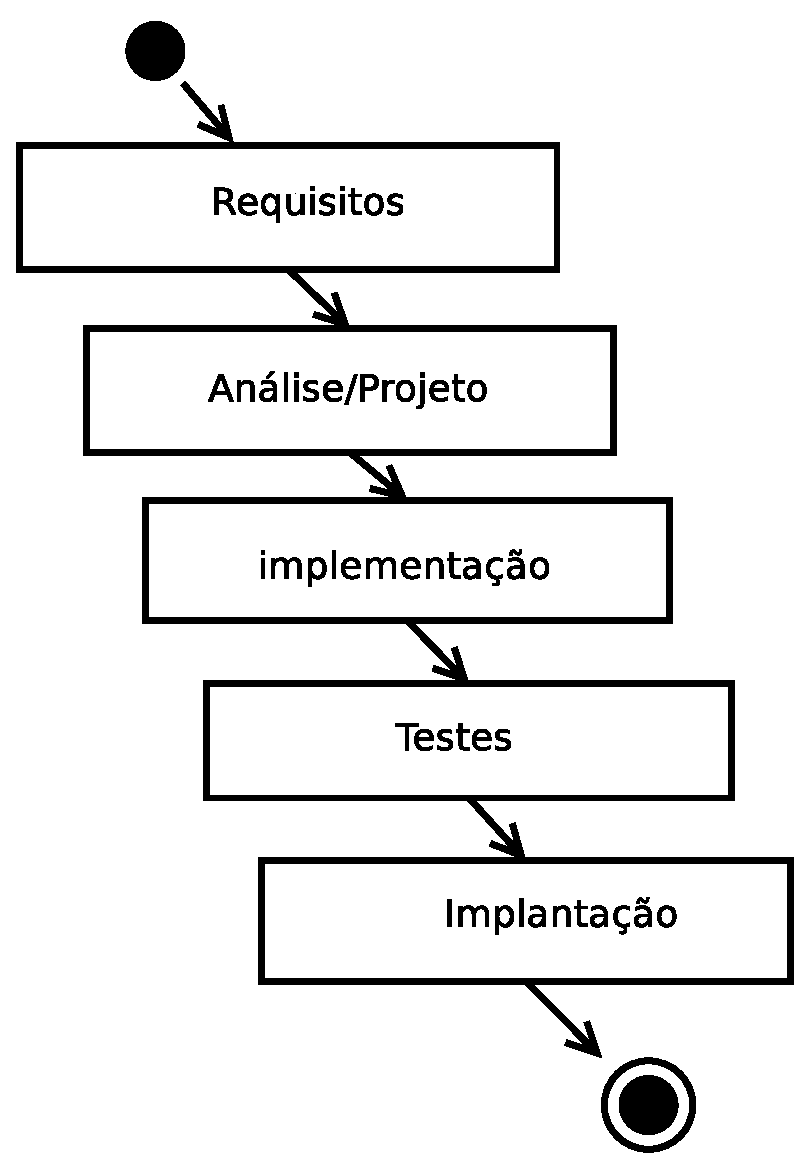
\includegraphics[width=4cm]{figuras/waterfall.eps}
	\caption{Exemplo de processo baseado no modelo \emph{waterfall}. Adaptado de \cite{Pressman2014}.}
	\label{waterfall}
\end{figure}

\begin{table}[ht]
	\caption{Comparando Modelos de Desenvolvimento de Software}
	\label{waterfall_x_agil}
	\ABNTEXfontereduzida
	\begin{tabular}{p{8cm}p{8cm}}
	\toprule
	\textit{Waterfall} & \textit{Ágil}\\
	\midrule
	\ABNTEXfontereduzida
	Prescritivo & Abstrato\\
	Documentação extensiva & Mínimo de documentação\\
	Sequencial & Contínuo\\
	Formal & Informal\\
	Foco no processo & Foco na comunicação\\
	Mudança gradual & Mudança rápida\\
	\bottomrule
	\end{tabular}
	\footnotesize Fonte:
	\cite{KristinRunyan2014}
\end{table}

